% \documentclass[14pt]{beamer}
\documentclass[handout,14pt]{beamer}

\usepackage{pgfpages}  % Uncomment one of these lines for X-on-1 printing
% \pgfpagesuselayout{4 on 1}[letterpaper, border shrink=5mm, landscape]
% \pgfpagesuselayout{2 on 1}[letterpaper, border shrink=5mm]

\usepackage{ifthen}
\newboolean{show_handout_comments}  % Uncomment one of the below
% \setboolean{show_handout_comments}{true}  % Show handout-only comments
\setboolean{show_handout_comments}{false}  % Hide comments

\usepackage{graphicx}
\usepackage{color}
\usepackage{enumerate}
\usepackage{bm}
\usepackage{listings}

\usepackage{booktabs}
\usepackage{multirow}

\usepackage{amsmath}
\usepackage{amssymb}
\usepackage{amsthm}
\usepackage{mathtools}
\usepackage{dsfont}
\usepackage{subfigure}


\usetheme{Madrid}
% \usecolortheme{}

\setbeamertemplate{enumerate items}[circle]  % standard enumeration
\setbeamertemplate{itemize items}[circle]  % default itemize
\setbeamertemplate{navigation symbols}{}

% Resuming lists across frames
\newcounter{savedenum}
\newcommand*{\saveenum}{\setcounter{savedenum}{\theenumi}}
\newcommand*{\resume}{\setcounter{enumi}{\thesavedenum}}

% Comments
\newcommand*{\comment}[2][red]{%
  \ifthenelse{\boolean{show_handout_comments}}{
  \only<beamer:0>{\textcolor{#1}{\footnotesize #2}}}{}}

% Boxes
\makeatletter
\newcommand*{\colbox}[2][black]{\textcolor{#1}{%
  \fbox{\normalcolor\m@th$\displaystyle#2$}}}
\makeatother

\newcommand*{\combox}[3][black]{%
  \mbox{\begin{tabular}[t]{@{}c@{}}
    $\colbox[#1]{\displaystyle#2}$\\
    \textcolor{#1}{\scriptsize #3}
    \end{tabular}}}

\newcommand*{\coltextbox}[2][black]{\textcolor{#1}{%
  \setlength{\fboxrule}{1pt}\fbox{\normalcolor#2}}}

\newcommand*{\answerbox}[2][black]{%
  \only<1|handout:0>{#2} \only<2>{\coltextbox[#1]{#2}}}

%%%%%%%%%%%%%%%%%%%%%%%%%%%%%%%%%%%%%%%%%%%%%%%%%%%%%%%%%%%%%%%%%%%%%%%%%%%%%%
% User-defined LaTeX commands
\DeclareMathOperator*{\Cov}{Cov}
\DeclareMathOperator*{\Var}{Var}
\DeclareMathOperator*{\argmax}{arg\,max}
\DeclareMathOperator*{\argmin}{arg\,min}
\DeclarePairedDelimiter{\abs}{\lvert}{\rvert}
\DeclarePairedDelimiter{\norm}{\lVert}{\rVert}
\newcommand*{\ttilde}{{\raise.17ex\hbox{$\scriptstyle\sim$}}}
\newcommand*{\foralls}{\ \forall \ }
\newcommand*{\E}{\mathbb E}
\newcommand*{\R}{\mathbb R}
\newcommand*{\I}{\mathds{1}}
\newcommand*{\Prob}{\mathbb P}
\newcommand*{\notorth}{\ensuremath{\perp\!\!\!\!\!\!\diagup\!\!\!\!\!\!\perp}}
\newcommand*{\orth}{\ensuremath{\perp\!\!\!\perp}}
\newcommand*{\dif}{\,\mathrm{d}}
\newcommand*{\Dif}[1]{\,\mathrm{d^#1}}
\newcommand*{\e}{\mathrm{e}}
\newcommand*{\m}[1]{\textbf{#1}}
\newcommand{\cond}{\;\ifnum\currentgrouptype=16 \middle\fi|\;}
\newcommand*{\bmath}[1]{\boldsymbol{#1}}
\newcommand*{\yestag}{\addtocounter{equation}{1}\tag{\theequation}}
\newcommand*{\notaligned}[1]{\noalign{$\displaystyle #1$}}

\makeatletter
\newsavebox{\mybox}\newsavebox{\mysim}
\newcommand*{\distas}[1]{%
  \savebox{\mybox}{\hbox{\kern3pt$\scriptstyle#1$\kern3pt}}%
  \savebox{\mysim}{\hbox{$\sim$}}%
  \mathbin{\overset{#1}{\kern\z@\resizebox{\wd\mybox}{\ht\mysim}{$\sim$}}}%
}
\makeatother
\newcommand*{\dist}{\sim}
\newcommand*{\distiid}{\distas{\text{i.i.d}}}

\newcommand*{\convas}[1]{\xrightarrow{#1}}
\newcommand*{\conv}{\convas{}}

\makeatletter
\def\moverlay{\mathpalette\mov@rlay}
\def\mov@rlay#1#2{\leavevmode\vtop{%
  \baselineskip\z@skip \lineskiplimit-\maxdimen
  \ialign{\hfil$\m@th#1##$\hfil\cr#2\crcr}}}
\newcommand{\charfusion}[3][\mathord]{
  #1{\ifx#1\mathop\vphantom{#2}\fi\mathpalette\mov@rlay{#2\cr#3}}
  \ifx#1\mathop\expandafter\displaylimits\fi}
\makeatother
\newcommand{\cupdot}{\charfusion[\mathbin]{\cup}{\cdot}}
\newcommand{\bigcupdot}{\charfusion[\mathop]{\bigcup}{\cdot}}
%%%%%%%%%%%%%%%%%%%%%%%%%%%%%%%%%%%%%%%%%%%%%%%%%%%%%%%%%%%%%%%%%%%%%%%%%%%%%%


\title[601 Final Project]{Hillary Clinton Emails}
\author[Leland Bybee, Roger Fan, Ryan Vaughn]{Leland Bybee, Roger Fan, Ryan Vaughn}
% \institute[]{}
\date{\today}


\begin{document}


\begin{frame}
\maketitle
\end{frame}

\begin{frame}{Some Interesting Topics}

\begin{table}[h]
\centering
\label{topic_top_words}
\scalebox{0.8}{
\begin{tabular}{cccccc}
\hline
Israel & Elections & Libya & Afghanistan & Int. Dev. & Obama \\
\hline
israel & democrat & libya & afghanistan & develop & presid \\
isra & republican & secur & pakistan & state & obama \\
peace & american & travel & afghan & support & said \\
palestinian & polit & libyan & militari & global & hous \\
netanyahu & parti & iraq & general & program & white \\
east & elect & embassi & karzai & effort & administr \\
negoti & obama & attack & offici & intern & polici \\
arab & percent & kill & war & work & aid \\
state & candid & march & forc & includ & advis

\end{tabular}
}
\end{table}

\end{frame}

\begin{frame}{Topic Importance Over Time}

\begin{figure}[h]
\centering
\subfigure[Israel]{\label{fig:t1}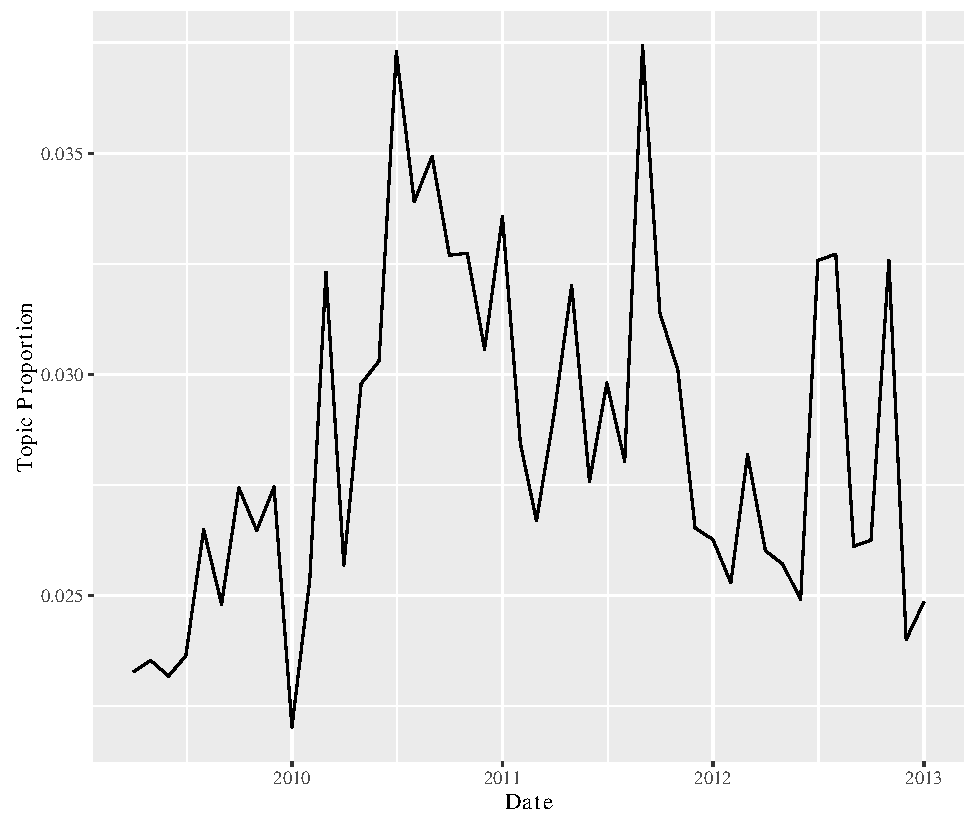
\includegraphics[width=29mm]{../images/time_plot6.pdf}}
\subfigure[Elections]{\label{fig:t2}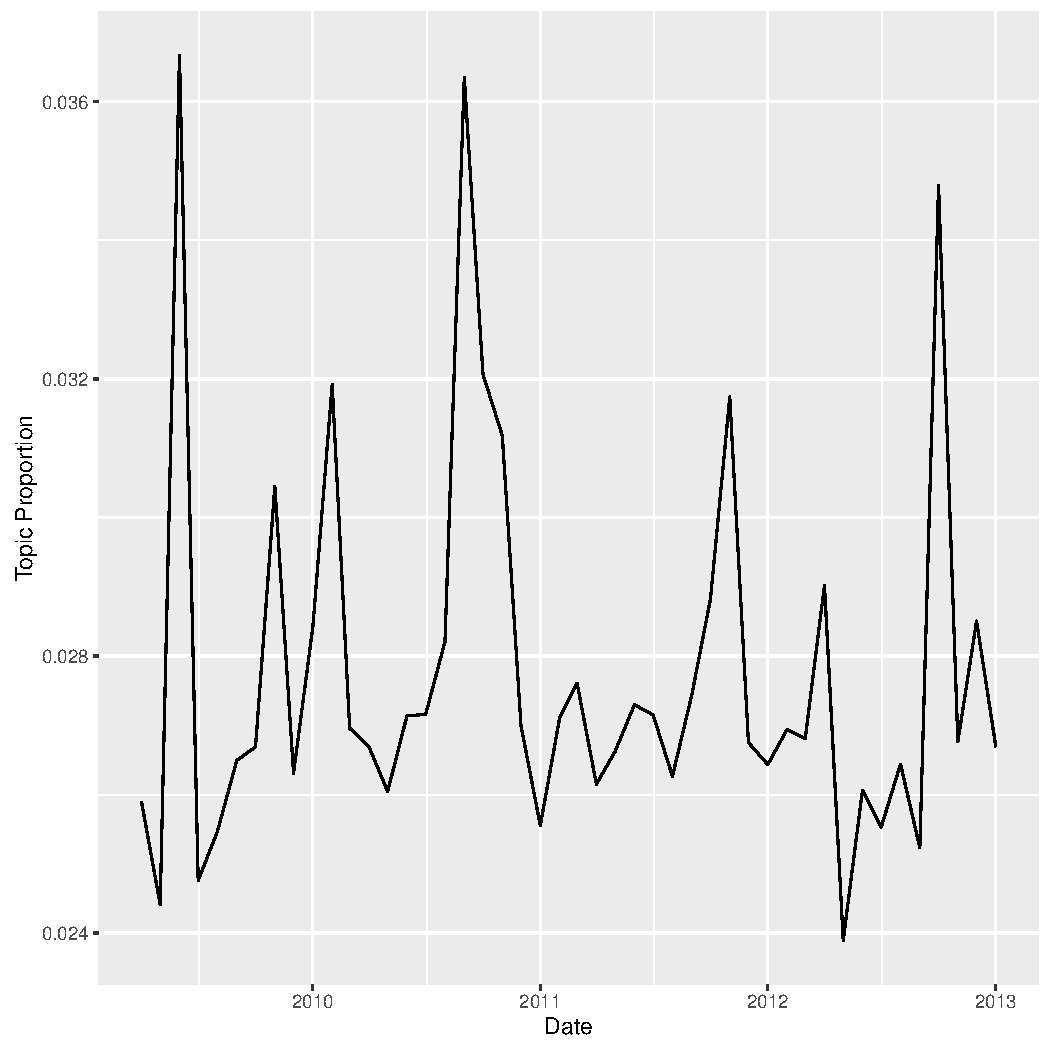
\includegraphics[width=29mm]{../images/time_plot11.pdf}}
\subfigure[Libya]{\label{fig:t3}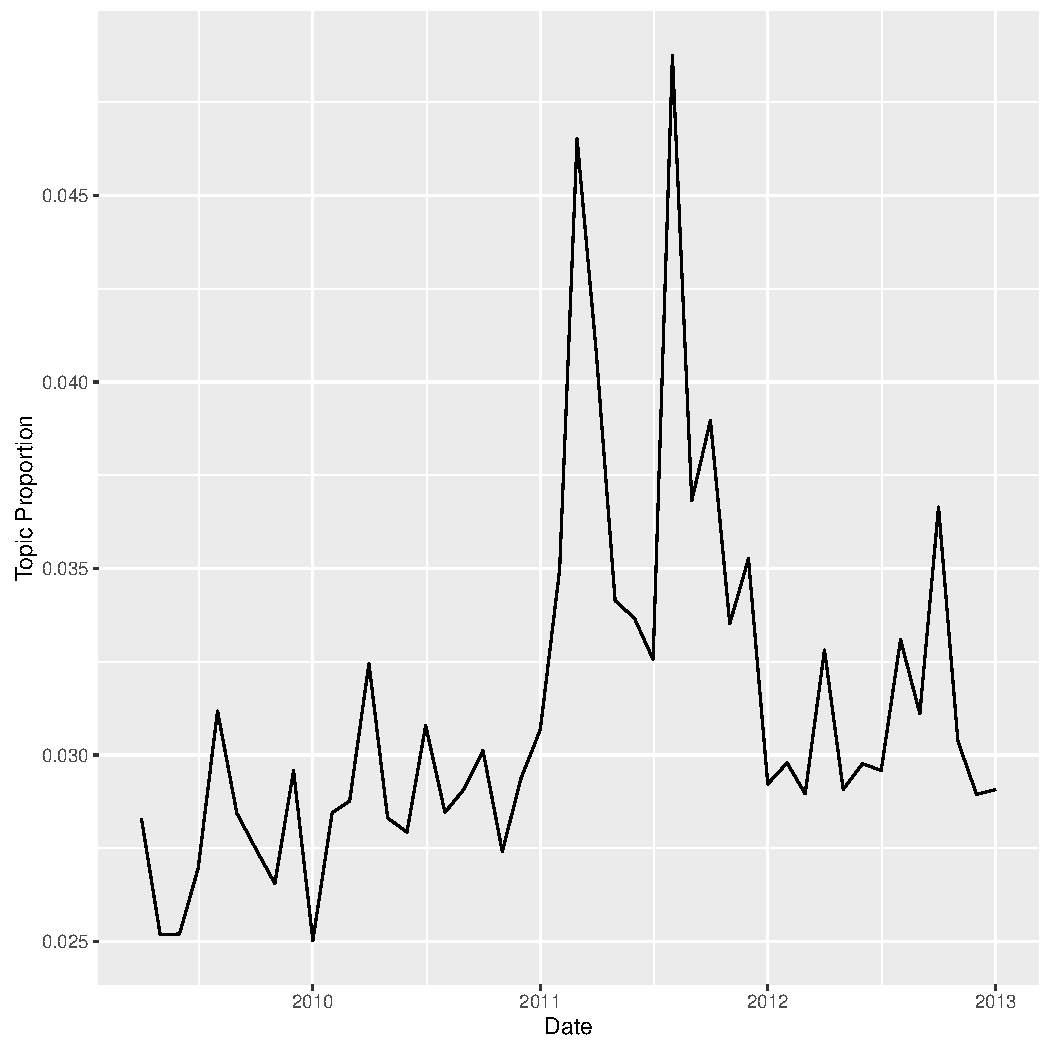
\includegraphics[width=29mm]{../images/time_plot18.pdf}}
\subfigure[Afghanistan]{\label{fig:t4}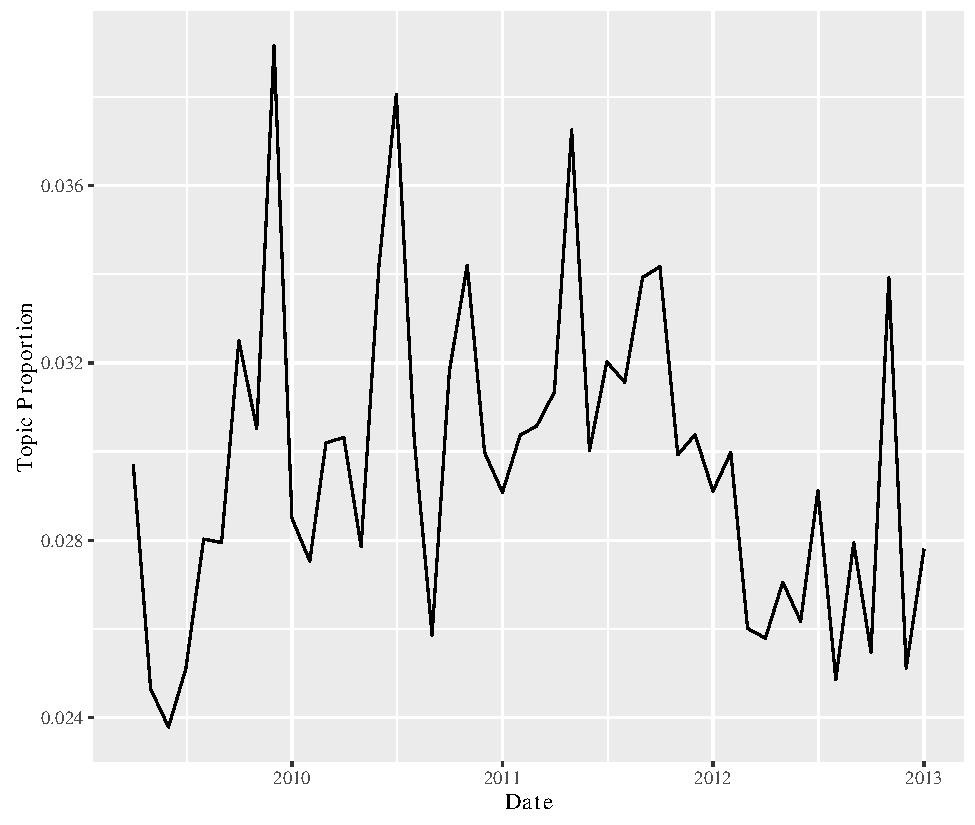
\includegraphics[width=29mm]{../images/time_plot27.pdf}}
\subfigure[Int. Dev.]{\label{fig:t5}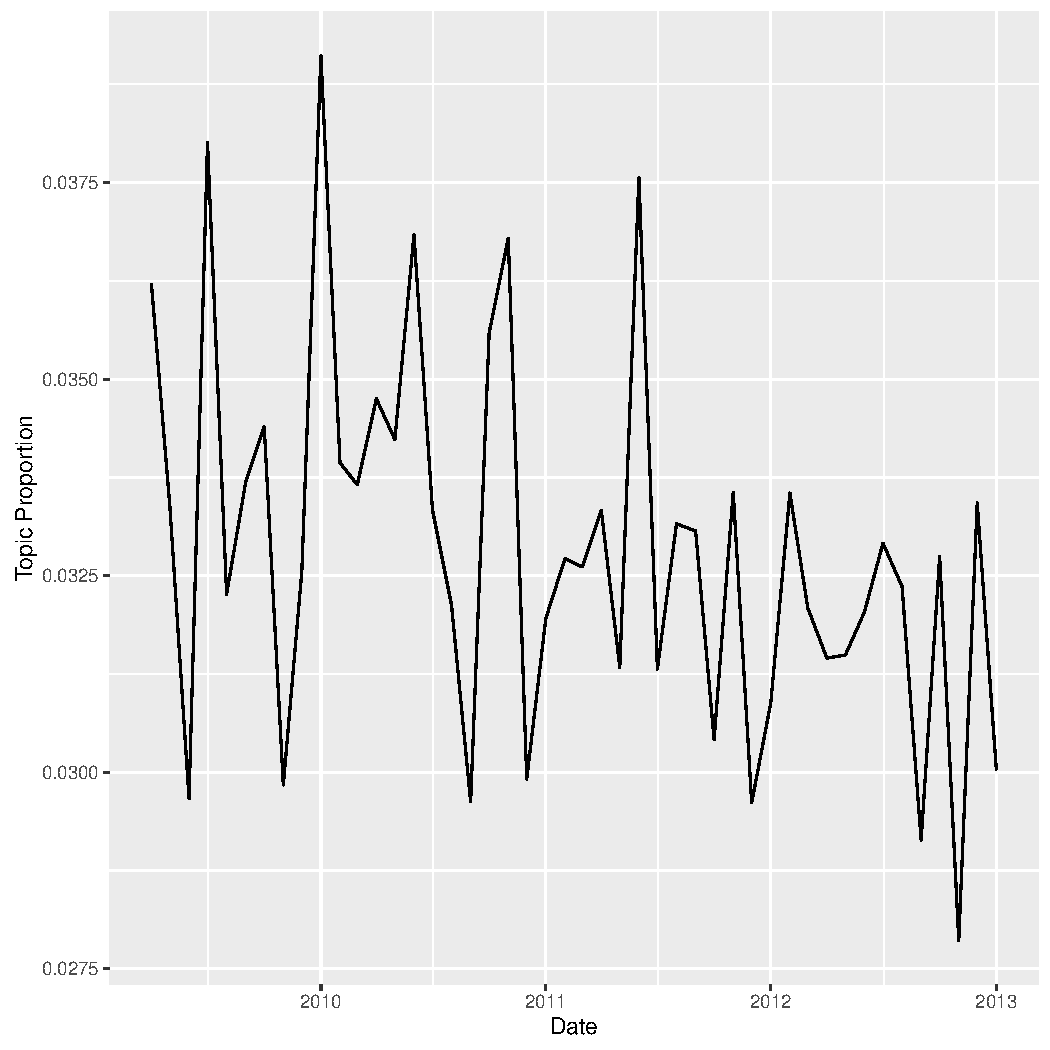
\includegraphics[width=29mm]{../images/time_plot23.pdf}}
\subfigure[Obama]{\label{fig:t6}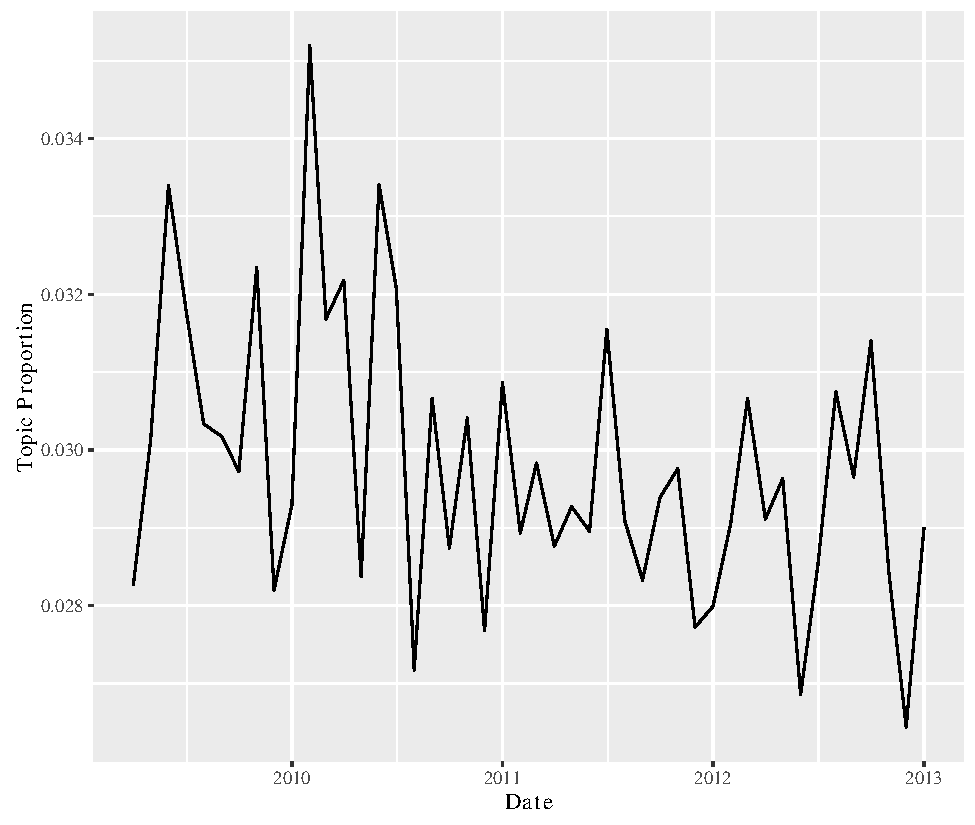
\includegraphics[width=29mm]{../images/time_plot25.pdf}}
\label{fig:topic_time_plots}
\end{figure}

\end{frame}

\begin{frame}{Who Says What?}

\begin{table}[h]
\centering
\label{topic_sources}
\scalebox{0.5}{
\begin{tabular}{cccccc}
\hline
Israel & Elections & Libya & Afghanistan & Int. Dev. & Obama \\
\hline
Sidney Blumenthal & SB & Huma Abedin & Judith McHale & JM & SB \\
(SB) & & (HA) & (JM) & & \\
\noalign{\vskip 7mm}
HA & Philippe Reines & Wendy Sherman & HA & Melanne Verveer & PR \\
& (PR) & (WS) & & (MV) & \\
\noalign{\vskip 7mm}
Jake Sullivan & JM & JS & MV & Anne-Marie & Cherly Mills \\
(JS) & & & & Slaughter (AMS) & (CM)\\
\noalign{\vskip 7mm}
AMS & CM & Monica Hanley & JS & CM & HA \\
& & (MH) & & & \\
\noalign{\vskip 7mm}
Hillary Clinton & HA & SB & Richard Verma & JS & HC \\
(HC) & & & (RV) & & \\

\end{tabular}
}
\end{table}

\end{frame}

\begin{frame}

\begin{table}[h]
\centering
\label{multinomial_results}
\scalebox{0.7}{
\begin{tabular}{ccc}
\hline
Source & Success Rate & Testing Observations \\
Hillary Clinton & 0.74 & 849 \\
Philippe Reines & 0.06 & 34 \\
Claire Coleman & 0.52 & 27 \\
Lauren Jiloty & 0.42 & 71 \\
Huma Abedin & 0.36 & 376 \\
Jake Sullivan & 0.23 & 410 \\
Sidney Blumenthal & 0.29 & 87 \\
Cherly Mills & 0.31 & 491 \\
Anne-Marie Slaughter & 0.36 & 42 \\
Monica Hanley & 0.09 & 53 \\
Judith McHale & 0.25 & 28 \\
Robert Russo & 0.00 & 10 \\
Richard Verma & 0.26 & 19 \\
Wendy Sherman & 0.08 & 12 \\
Melanne Verveer & 0.30 & 30 \\
Lona Valmoro & 0.34 & 41
\end{tabular}
}
\end{table}


\end{frame}

\end{document}
